\documentclass[11pt,oneside]{article}
\usepackage[T1]{fontenc}
\usepackage[utf8]{inputenc}
%\DeclareUnicodeCharacter{00A0}{ }
\usepackage[adobe-utopia]{mathdesign}

\usepackage{amsmath}
\usepackage[francais]{babel}
\usepackage[dvips]{graphicx}
%\usepackage{here}
\usepackage{framed}
\usepackage[normalem]{ulem}
\usepackage{fancyhdr}
\usepackage{titlesec}
\usepackage{vmargin}

\usepackage{amsmath}
\usepackage{ifthen}
\usepackage{multirow}
\usepackage{multicol} % Portions de texte en colonnes

%\usepackage{xltxtra} % Logo XeLaTeX
%\usepackage{pst-solides3d}
\usepackage{color}
%\usepackage{colortbl}
\usepackage{titletoc} % Pour la mise en forme de la table des matières

%\usepackage[crop=off]{auto-pst-pdf}
%\usepackage{bclogo}


%\usepackage{longtable}
%\usepackage{flafter}%floatants après la référence
%\usepackage{pst-solides3d}
%\usepackage{pstricks}
%\usepackage{minitoc}
%\setcounter{minitocdepth}{4}
%\usepackage{draftcopy}% "Brouillon"
%\usepackage{floatflt}
%\usepackage{psfrag}
%\usepackage{listings} % Permet d'insérer du code de programmation
%\usepackage{lmodern}
%\usepackage[adobe-utopia,uppercase=upright,greeklowercase=upright]{mathdesign}
%\usepackage{minionpro}
%\usepackage{pifont}
%\usepackage{amssymb}
%\usepackage[francais]{varioref}

\setmarginsrb{1.5cm}{1cm}{1cm}{1.5cm}{1cm}{1cm}{1cm}{1cm}

\definecolor{gris25}{gray}{0.75}
\definecolor{bleu}{RGB}{18,33,98}
\definecolor{bleuf}{RGB}{42,94,171}
\definecolor{bleuc}{RGB}{231,239,247}
\definecolor{rougef}{RGB}{185,18,27}
\definecolor{rougec}{RGB}{255,230,231}
\definecolor{vertf}{RGB}{103,126,82}
\definecolor{vertc}{RGB}{220,255,191}
\definecolor{violetf}{RGB}{112,48,160}
\definecolor{violetc}{RGB}{230,224,236}
\definecolor{jaunec}{RGB}{220,255,191}
\usepackage[final]{pdfpages} 
\usepackage[%
    pdftitle={TD Conception},
    pdfauthor={Xavier Pessoles},
    colorlinks=true,
    linkcolor=blue,
    citecolor=magenta]{hyperref}



% \makeatletter \let\ps@plain\ps@empty \makeatother
%% DEBUT DU DOCUMENT
%% =================
\sloppy
\hyphenpenalty 10000

\newcommand{\Pointilles}[1][3]{%
\multido{}{#1}{\makebox[\linewidth]{\dotfill}\\[\parskip]
}}


\begin{document}


\newboolean{prof}
\setboolean{prof}{false}
%------------- En tetes et Pieds de Pages ------------
\pagestyle{fancy}
\renewcommand{\headrulewidth}{0pt}

\fancyhead{}
\fancyhead[L]{%
\begin{minipage}[c]{1.6cm}

\includegraphics[width=1.5cm]{png/logo_ptsi.png}%
\end{minipage}
\rule{2cm}{.5pt}
}

\fancyhead[C]{\rule{11cm}{.5pt}}

\fancyhead[R]{%
\begin{minipage}[c]{3cm}
\begin{flushright}
\footnotesize{\textit{\textsf{Sciences Industrielles\\ de l'Ingénieur}}}%
\end{flushright}
\end{minipage}
}

\renewcommand{\footrulewidth}{0.2pt}

\fancyfoot[C]{\footnotesize{\bfseries \thepage}}
\fancyfoot[L]{\footnotesize{2012 -- 2013} \\ X. \textsc{Pessoles}}
\ifthenelse{\boolean{prof}}{%
\fancyfoot[R]{\footnotesize{TD -- CI 4 -- Conception des mécanismes -- P}}
}{%
\fancyfoot[R]{\footnotesize{TD -- CI 4 -- Conception des mécanismes}}
}


%\begin{center}
%\textit{Centre d'intérêt}
%\end{center}


\begin{center}
 \huge\textsc{CI 4 -- Conception des mécanismes}
\end{center}


\begin{center}
 \large\textsc{Frein hydraulique d'un treuil}
\end{center}
\vspace{.5cm}

%
%\begin{minipage}[c]{.45\linewidth}
%\begin{center}
%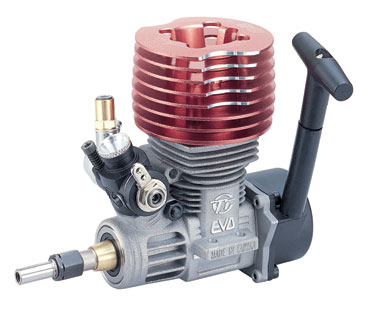
\includegraphics[height=3cm]{png/moteur}
%
%\textit{Moteur de modélisme}
%\end{center}
%\end{minipage}\hfill
%\begin{minipage}[c]{.45\linewidth}
%\begin{center}
%\includegraphics[height=4cm]{png/moteur_3D}
%
%\textit{Représentation d'un moteur de modélisme}
%\end{center}
%\end{minipage}


\section*{Caractéristiques techniques}

\begin{minipage}[c]{.47\linewidth}

\textbf{Moteur hydraulique :}
\begin{itemize}
\item Pression d'alimentation : $p_1 = 145 \; bars$
\item Fréquence de rotation : $N_1 = 1500 \; tr/min$
\end{itemize}


\textbf{Réducteur -- Pignons droits : }
\begin{itemize}
\item $Z_1 = 11$;
\item $Z_4" = 15$;
\item $Z_4' = 13$;
\item $Z_9 = 39$.
\end{itemize}

\textbf{Tambour : }
\begin{itemize}
\item câble (sur trois couches) : $\phi = 10,5\;mm$;
\item diamètre mini du tambour : $D_2 = 182\; mm$;
\item effort de traction maximal : $F_5 = 1\,500 \; daN$.
\end{itemize}


\end{minipage}\hfill
\begin{minipage}[c]{.47\linewidth}

\textbf{Frein à disque : }
\begin{itemize}
\item diamètre extérieur des surfaces frottantes : $D_e = 134\; mm$;
\item diamètre intérieur des surfaces frottantes : $D_i = 78\; mm$;
\item facteur de frottement : $f = 0,3$;
\item diamètre extérieur du piston 10 : $d_e = 100 \; mm$;
\item diamètre intérieur du piston 10 : $d_i = 74 \;mm$;
\item course du piston 10 avec garnitures neuves 11 : $1 \;mm$;
\item usure possible de chaque garniture 11 : $2\; mm$;
\item dimensions des rondelles Belleville formant le ressort 12 : $63 x 31 x 2$;
\item rigidité (constante) d'une rondelle : $4064 \; N / mm$;
\item course d'une rondelle : $1,8 \; mm$.
\end{itemize}

\end{minipage}



\section*{Critères d'évaluation}

Au vu du schéma technologique, les fonctions suivantes sont à réaliser :
\begin{itemize}
\item liaison pivot de l'arbre 1 avec le bâti. Cette liaison permet d'assurer le guidage de l'arbre à son extrémité gauche;
\item liaison pivot glissant du piston 10 avec le bâti. Le piston permettant de desserrer le frein hydraulique;
\item liaison glissière des disques 11 par rapport à l'arbre 1;
\item liaison glissière de la plaque 14 par rapport à 3;
\item le système de freinage comprenant l'arrivée du fluide sous pression ($P_{10}$), la compression des ressorts 12, l'étanchéité au niveau du piston.
\end{itemize}

Comme pour tout système mécanique, il faut prendre garde : 
\begin{itemize}
\item à ce que le système s'assemble;
\item à ce que les pièces puissent se fabriquer (par moulage, forgeage, usinage);
\item à préciser les ajustements;
\item à ce que le tracé soit soigné.
\end{itemize}

\end{document}